% Drawing 161-6/01-14 -- folder 161-6, batch 01, archive page 19 (PDF page 20).
% Transcription: au bord droit, au crayon, un cône vu de côté : un long axe épais, d'où part à mi-hauteur, vers la droite, une lentille (la base) ; un trait fin joint le haut de l'axe au bord de la base ; du même point de l'axe partent deux flèches pâles, et une plage noircie longe l'axe jusqu'en bas ; légendes « $1$ », « $\alpha$ », « $\cos\alpha$ », « $72^{\circ}$ » ; une flèche courbe monte de la base vers la formule « $2\rho\sin\frac{\theta}{2}$ ».
% Kind: cone seen from the side, with cos alpha and an angle of 72 degrees. Method 2 (schematic redraw from the facsimile). Status: partial.
% Notes: Drawn: the heavy axis from the top to the bottom point; the point on it from which the base leaves; the base as a lens (thin upper side, heavy lower arc) ending at the right corner; the thin pencil side from the top to that corner; the two faint arrows from the same point of the axis, towards the right and towards the lower right; the blackened sliver along the lower half of the axis (hatched); the curved arrow rising from the base. Labels turned as on the page: 1 and alpha beside the upper part of the axis, cos alpha at its left lower down, 72° between the two faint arrows. Still differs: the axis is several strokes gone over and is drawn as one; a small scribble where the curved arrow starts (perhaps « cos ») and a « 1 » near the lower end of the axis are not read with certainty and are left out; which angle the 72° measures was said not to be marked by an arc (see below). Redrawn 2026-11-12 (issue 128): to check again. 2026-11-14, Claude Opus 5.5, issue 147 second pass: on the 400 dpi scan the blackened sliver is a solid pencil shading, not separate strokes, so it is drawn as a grey fill bounded by its two edges read on the page (its right edge bowed, its left edge running close to the axis), in place of the earlier hatched patch; the curved arrow redrawn through points on its ink from its start on the lens (it bulged one to two units to the left); a faint pencil arc under the lens, between the two faint arrows, which the earlier redraw left out, is added: it marks an angle at the point where the two faint arrows leave, and 72° is written beside it. Overlay with the local TikZ interpreter (not compiled: no TeX in the session): every stroke and the shading lie on their ink to within about one unit. Still differs: only the small scribble where the curved arrow starts (perhaps « cos ») and the « 1 » near the lower end of the axis, not read with certainty and left out.
% Coordinates: 1 unit = 1 mm = 1/100 of the crop width; labels turned as on the page (leaf written in two directions (the pencil writing runs down the scanned page); drawn as the scan shows it, labels turned as on the page) (bbox in page fractions: [0.83, 0.325, 0.97, 0.453]).
% Redrawn by Claude (claude-fable-5-2), issue #128, 2026-11-12; not checked by a human; not compiled (no TeX in the session); overlay-checked on the scan by Claude Opus 5.5, issue #147, 2026-11-13, not compiled (no TeX in the session).
% Rights: reproduces part of the work -- behind RENDER_TRANSCRIPTS, never published by itself.
\documentclass[tikz,border=3pt]{standalone}
\usepackage{amsmath,amssymb}
\usetikzlibrary{patterns,arrows.meta}
\tikzset{pencil/.style={black!45}, struck/.style={black!35}, mpt/.style={circle,draw,inner sep=1.3pt}, pt/.style={circle,fill,inner sep=0.9pt}, opt/.style={circle,draw,fill=white,inner sep=1.1pt}}
\begin{document}
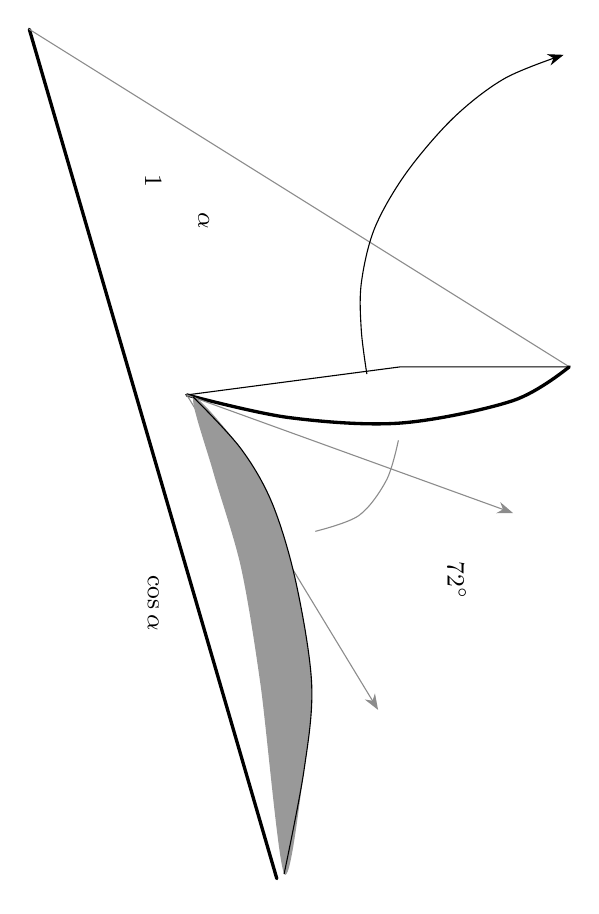
\begin{tikzpicture}[x=1mm,y=1mm,line cap=round,line join=round,font=\small]
\draw[very thick] (17.14,-11.76) -- (48.57,-119.62);
\draw[pencil] (17.14,-11.76) -- (85.71,-54.62);
\draw (37.14,-58.19) -- (64.29,-54.62) -- (85.71,-54.62);
\draw[very thick] plot[smooth, tension=0.55] coordinates {(37.14,-58.19) (50,-61.05) (64.29,-61.76) (78.57,-58.91) (85.71,-54.62)};
\draw[pencil,-{Stealth[length=2mm]}] (37.14,-58.19) -- (78.57,-73.19);
\draw[pencil,-{Stealth[length=2mm]}] (37.14,-58.19) -- (61.43,-98.19);
\fill[black!40] plot[smooth cycle, tension=0.5] coordinates {(38,-58.5) (44,-65) (48,-72) (51,-82) (53,-95) (52,-106) (49.5,-119) (46.5,-95) (44,-80) (40.5,-68)};
\draw plot[smooth, tension=0.55] coordinates {(38,-58.5) (44,-65) (48,-72) (51,-82) (53,-95) (52,-106) (49.5,-119)};
\draw[pencil] plot[smooth, tension=0.55] coordinates {(53.5,-75.5) (59,-73.5) (62.5,-69) (64,-64)};
\draw[-{Stealth[length=2mm]}] plot[smooth, tension=0.55] coordinates {(60,-55.5) (59.3,-50) (59.3,-44) (61,-37) (65,-30) (71,-23) (77.5,-18) (85,-15)};
\node[inner sep=1pt,rotate=-90] at (32.86,-31.05) {\small $1$};
\node[inner sep=1pt,rotate=-90] at (39.29,-36.05) {\small $\alpha$};
\node[inner sep=1pt,rotate=-90] at (32.86,-84.62) {\small $\cos\alpha$};
\node[inner sep=1pt,rotate=-90] at (71.43,-81.76) {\small $72^{\circ}$};
\end{tikzpicture}
\end{document}
